\documentclass[a0paper,portrait]{baposter}

\usepackage{relsize}		% For \smaller
\usepackage{url}			% For \url
\usepackage{adjustbox}
% \usepackage{epstopdf}	% Included EPS files automatically converted to PDF to include with pdflatex

%%% Global Settings %%%%%%%%%%%%%%%%%%%%%%%%%%%%%%%%%%%%%%%%%%%%%%%%%%%%%%%%%%%

\graphicspath{{pix/}}	% Root directory of the pictures 
% \tracingstats=2			% Enabled LaTeX logging with conditionals

%%% Color Definitions %%%%%%%%%%%%%%%%%%%%%%%%%%%%%%%%%%%%%%%%%%%%%%%%%%%%%%%%%

\definecolor{bordercol}{RGB}{40,40,40}
\definecolor{headercol1}{RGB}{186,215,230}
\definecolor{headercol2}{RGB}{80,80,80}
\definecolor{headerfontcol}{RGB}{0,0,0}
\definecolor{boxcolor}{RGB}{186,215,230}

%%%%%%%%%%%%%%%%%%%%%%%%%%%%%%%%%%%%%%%%%%%%%%%%%%%%%%%%%%%%%%%%%%%%%%%%%%%%%%%%
%%% Utility functions %%%%%%%%%%%%%%%%%%%%%%%%%%%%%%%%%%%%%%%%%%%%%%%%%%%%%%%%%%

%%% Save space in lists. Use this after the opening of the list %%%%%%%%%%%%%%%%
\newcommand{\compresslist}{
	\setlength{\itemsep}{1pt}
	\setlength{\parskip}{0pt}
	\setlength{\parsep}{0pt}
}

%%%%%%%%%%%%%%%%%%%%%%%%%%%%%%%%%%%%%%%%%%%%%%%%%%%%%%%%%%%%%%%%%%%%%%%%%%%%%%%
%%% Document Start %%%%%%%%%%%%%%%%%%%%%%%%%%%%%%%%%%%%%%%%%%%%%%%%%%%%%%%%%%%%
%%%%%%%%%%%%%%%%%%%%%%%%%%%%%%%%%%%%%%%%%%%%%%%%%%%%%%%%%%%%%%%%%%%%%%%%%%%%%%%

\begin{document}
\typeout{Poster rendering started}

%%% Setting Background Image %%%%%%%%%%%%%%%%%%%%%%%%%%%%%%%%%%%%%%%%%%%%%%%%%%
\background{
	\begin{tikzpicture}[remember picture,overlay]%
	\draw (current page.north west)+(-2em,2em) node[anchor=north west]
	{\includegraphics[height=1.1\textheight]{images/background.pdf}};
	\end{tikzpicture}
}

%%% General Poster Settings %%%%%%%%%%%%%%%%%%%%%%%%%%%%%%%%%%%%%%%%%%%%%%%%%%%
%%%%%% Eye Catcher, Title, Authors and University Images %%%%%%%%%%%%%%%%%%%%%%
\begin{poster}{
	grid=false,
	% Option is left on true though the eyecatcher is not used. The reason is
	% that we have a bit nicer looking title and author formatting in the headercol
	% this way
	%eyecatcher=false, 
	borderColor=bordercol,
	headerColorOne=headercol1,
	headerColorTwo=headercol2,
	headerFontColor=headerfontcol,
	% Only simple background color used, no shading, so boxColorTwo isn't necessary
	boxColorOne=boxcolor,
	headershape=roundedright,
	headerfont=\Large\sf\bf,
	textborder=rectangle,
	background=user,
	headerborder=open,
  boxshade=plain
}
%%% Eye Cacther %%%%%%%%%%%%%%%%%%%%%%%%%%%%%%%%%%%%%%%%%%%%%%%%%%%%%%%%%%%%%%%
{
	Eye Catcher, empty if option eyecatcher=false - unused
}
%%% Title %%%%%%%%%%%%%%%%%%%%%%%%%%%%%%%%%%%%%%%%%%%%%%%%%%%%%%%%%%%%%%%%%%%%%
{\sf\bf
	Topology-resolved quantum volume
}
%%% Authors %%%%%%%%%%%%%%%%%%%%%%%%%%%%%%%%%%%%%%%%%%%%%%%%%%%%%%%%%%%%%%%%%%%
{
	\vspace{1em} Henrijs Kravals, Maksims Dimitrijevs\\
	{\smaller henrijs.kravals@lu.lv, maksims.dimitrijevs@lu.lv}
}
%%% Logo %%%%%%%%%%%%%%%%%%%%%%%%%%%%%%%%%%%%%%%%%%%%%%%%%%%%%%%%%%%%%%%%%%%%%%
{
% The logos are compressed a bit into a simple box to make them smaller on the result
% (Wasn't able to find any bigger of them.)
\setlength\fboxsep{0pt}
    \begin{minipage}{14em}
        \centering
        \includegraphics[width=0.7\linewidth]{images/logo.pdf}
    \end{minipage}
}

\headerbox{Problem}{name=problem,column=0,row=0}{
\begin{itemize}\compresslist
\item NISQ devices have useful scale, but are limited by noise and lack fault tolerance.
\item Performance depends on qubit quality, connectivity, and compilation overhead.
\item Therefore, system-level benchmarks are needed in addition to gate-level metrics.
\end{itemize}
 One such benchmark is quantum volume, which assesses only a limited subset of best-quality qubits within a quantum processor. We study how quantum volume depends on \emph{where} a circuit is placed on a chip, not only on the chip as a whole.
}

\headerbox{Quantum volume}{name=definitions,column=0,below=problem}{
    Quantum volume (QV) is a \textbf{system level benchmark}. The QV is a single number figure of merit used to evaluate universal gate-based quantum computers. 

    \begin{center}
        \includegraphics[width=\linewidth]{images/qv-process.png}

        \small \textbf{The QV circuit~\cite{qv_benchmark_zoo}}
    \end{center}

    If the quantum computer samples a distribution from the \textbf{heavy set of outputs} (simulated classically) with probability $> 2/3$, it validates the corresponding quantum volume score of $2^n$. The confidence interval for this evaluation is set to $2\sigma$ ($97.7\%$).
}

\headerbox{\emph{Heavy set of outputs}}{name=models,column=0,below=definitions}{
    Let $\mathbf{Q}$ be a random circuit drawn from a suitable ensemble acting on $n$ qubits. The quantum state after executing the circuit is denoted $|\psi\rangle$. Each possible output state $x\in\{0,1\}^n$ is measured with probability $|\langle x|\psi\rangle|^2$. The set of output states with a probability greater than the median constitutes the heavy set of outputs associated with the quantum circuit $\mathbf{Q}$.
}

\headerbox{References}{name=references,column=0,below=models}{
\smaller
\vspace{-0.4em} 										% Save some space at the beginning
\bibliographystyle{plain}							% Use plain style
\renewcommand{\section}[2]{\vskip 0.05em}		% Omit "References" title
\begin{thebibliography}{1}							% Simple bibliography with widest label of 1
\itemsep=-0.01em										% Save space between the separation
\setlength{\baselineskip}{0.4em}					% Save space with longer lines
\bibitem{qv_benchmark_zoo}
Quantum Benchmark Zoo:
\emph{Quantum Volume}.
Available at: \url{https://quantumbenchmarkzoo.org}
(accessed 2026-04-12).
\end{thebibliography}
}

\headerbox{Acknowledgements}{name=acknowledgements,column=0,below=references, above=bottom}{
\smaller						% Make the whole text smaller
\vspace{-0.4em}			% Save some space at the beginning
This work was supported by the University of Latvia student research funding, aimed at promoting the involvement of 1st and 2nd year bachelor-level and short-cycle students in research activities at the Faculty of Science and Technology (EZTF). 
} 

\headerbox{Research methodology}{name=density,span=2,column=1,row=0}{
We benchmarked QV on the IBM Marrakesh device using calibration data and the coupling graph from Qiskit. First, we construct a noisy quantum simulator from the extracted data. Then we enumerate all connected subgraphs of size $n \leq 6$ and run QV circuits on each subgraph. Finally, we compute the heavy output probability and confidence for each placement.
}

\headerbox{Productivity of qubit subsets varies significantly}
{name=degreeDistribution,span=2,column=1,below=density,above=bottom}{

	\begin{minipage}[t]{0.49\linewidth}
	\vspace{0pt}
		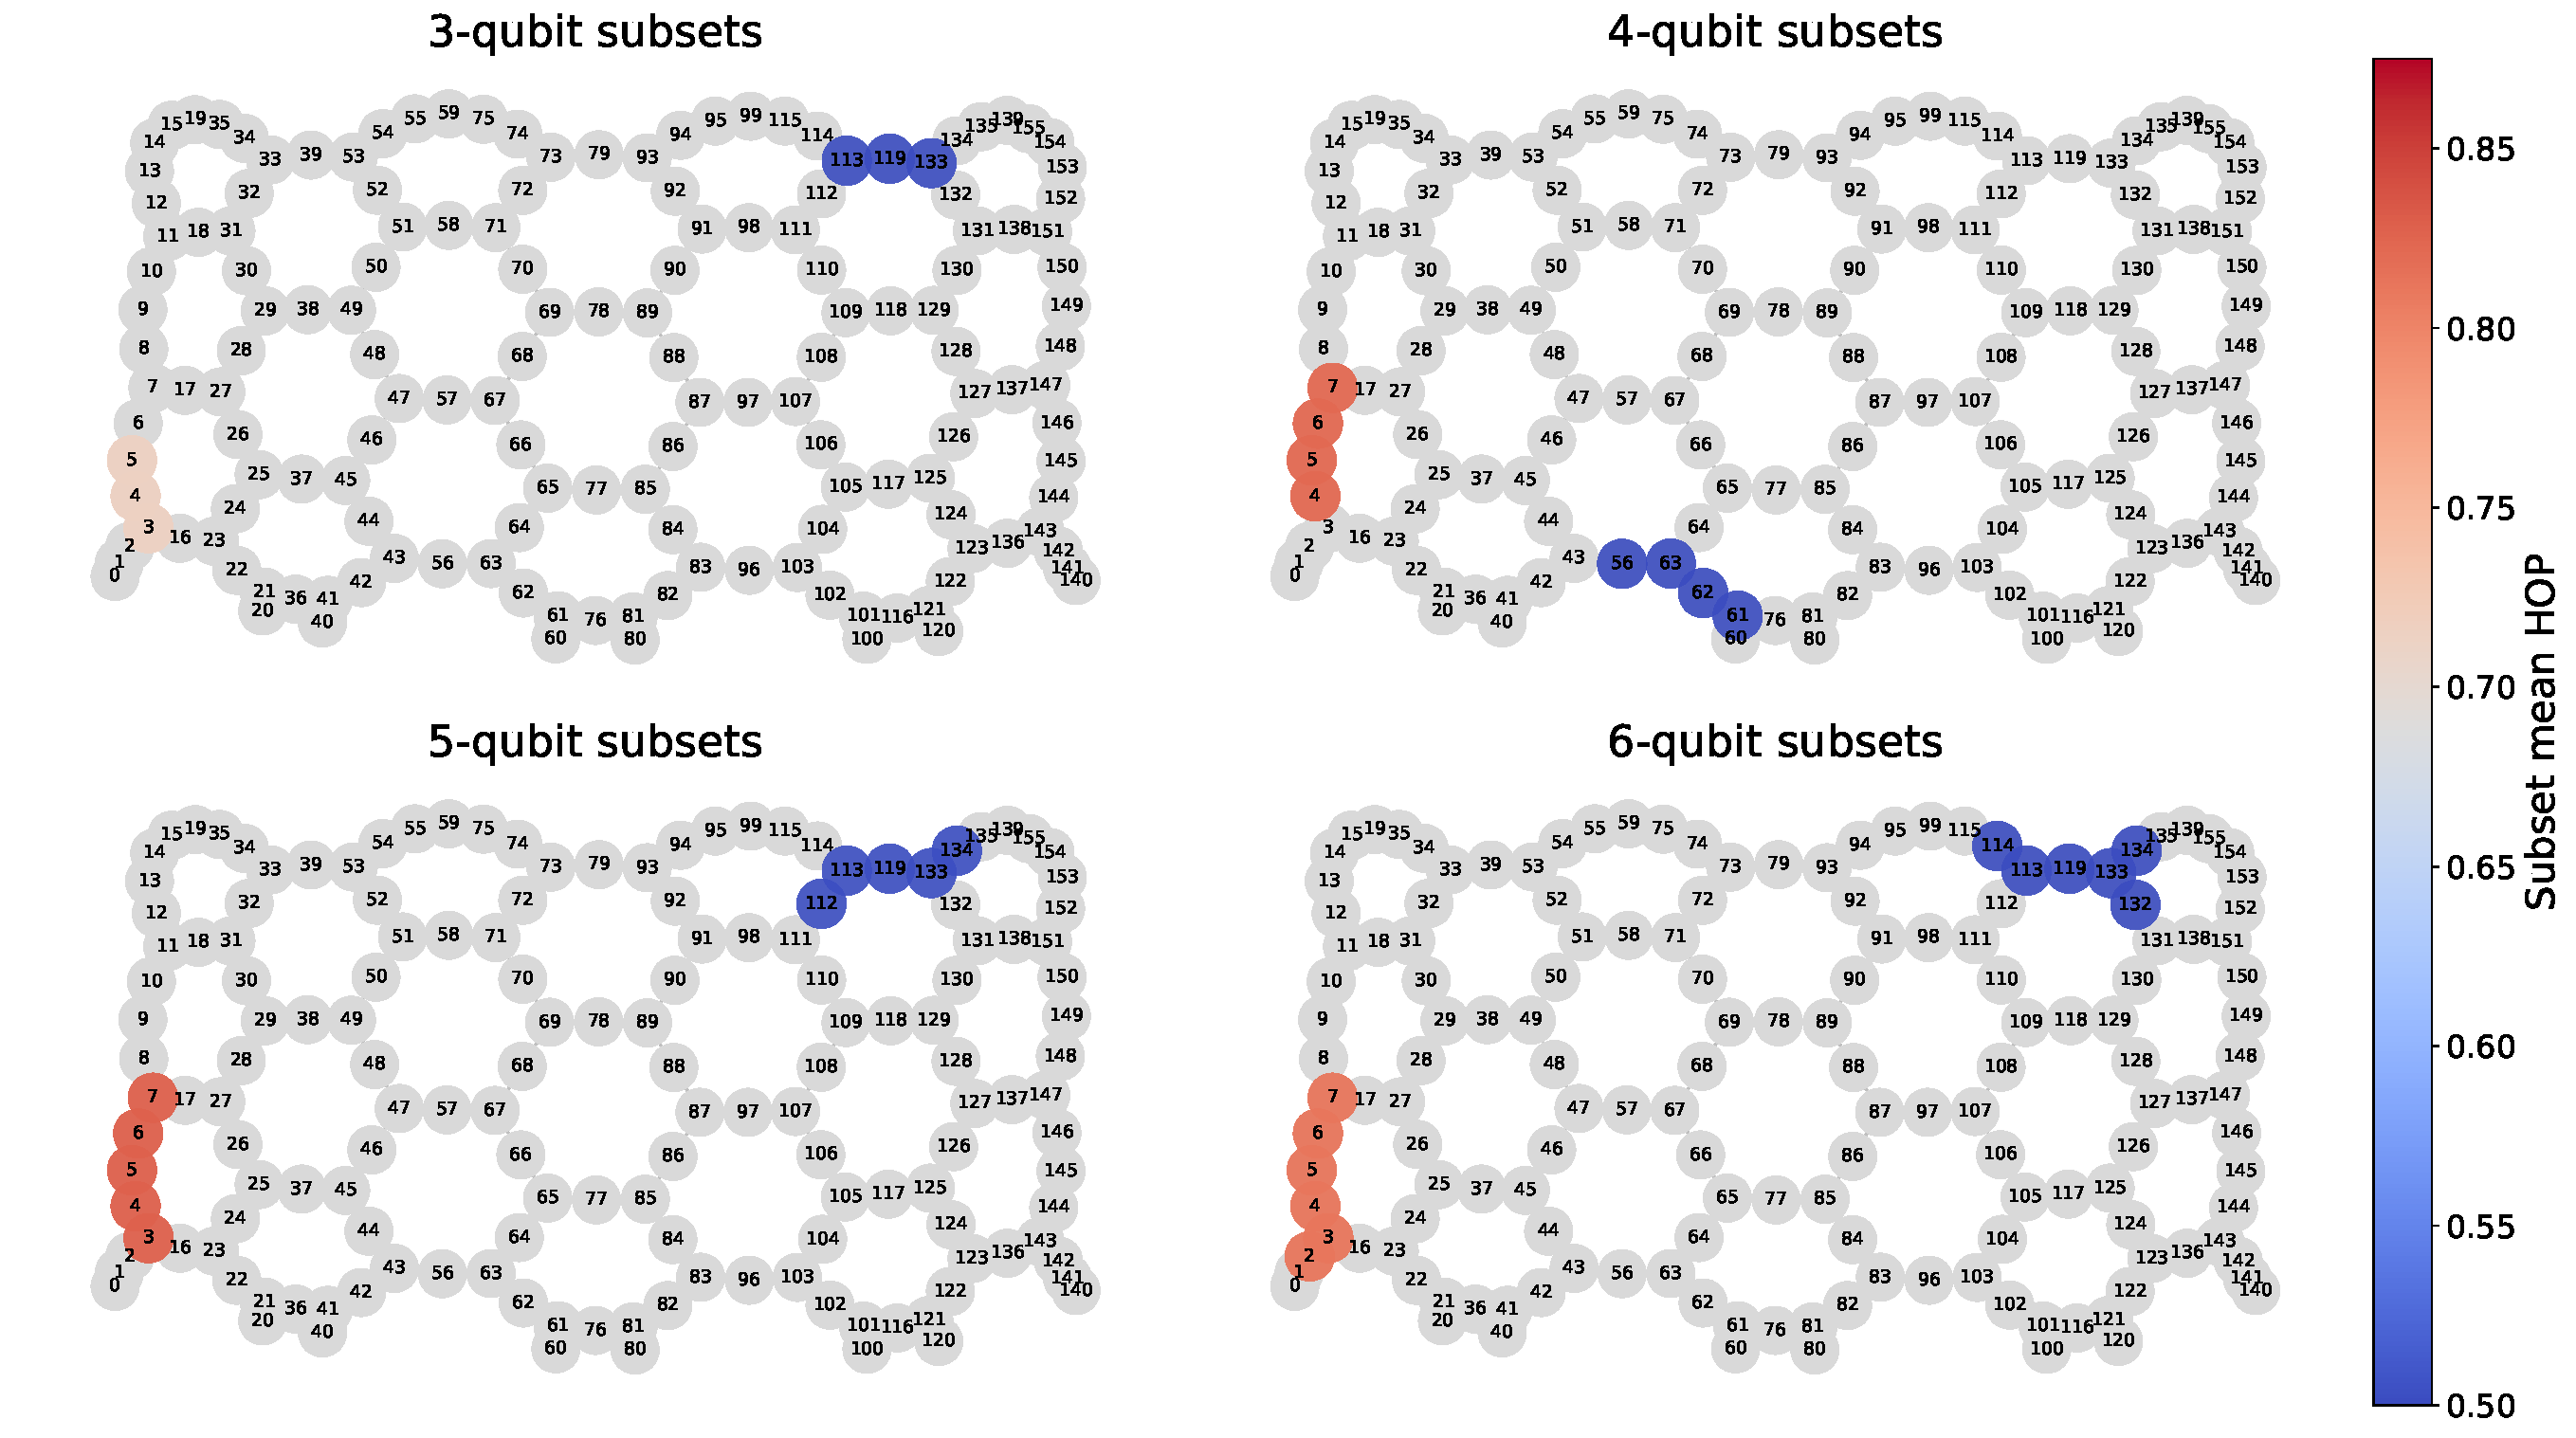
\includegraphics[width=\linewidth]{../results/best_worst_grid.pdf}
		\small \textbf{The best and worst HOP wise performing subsets of different subset sizes.} Comparison makes the topology dependence clear: some regions of the chip are much better than others.

		\vspace{0.6em}

		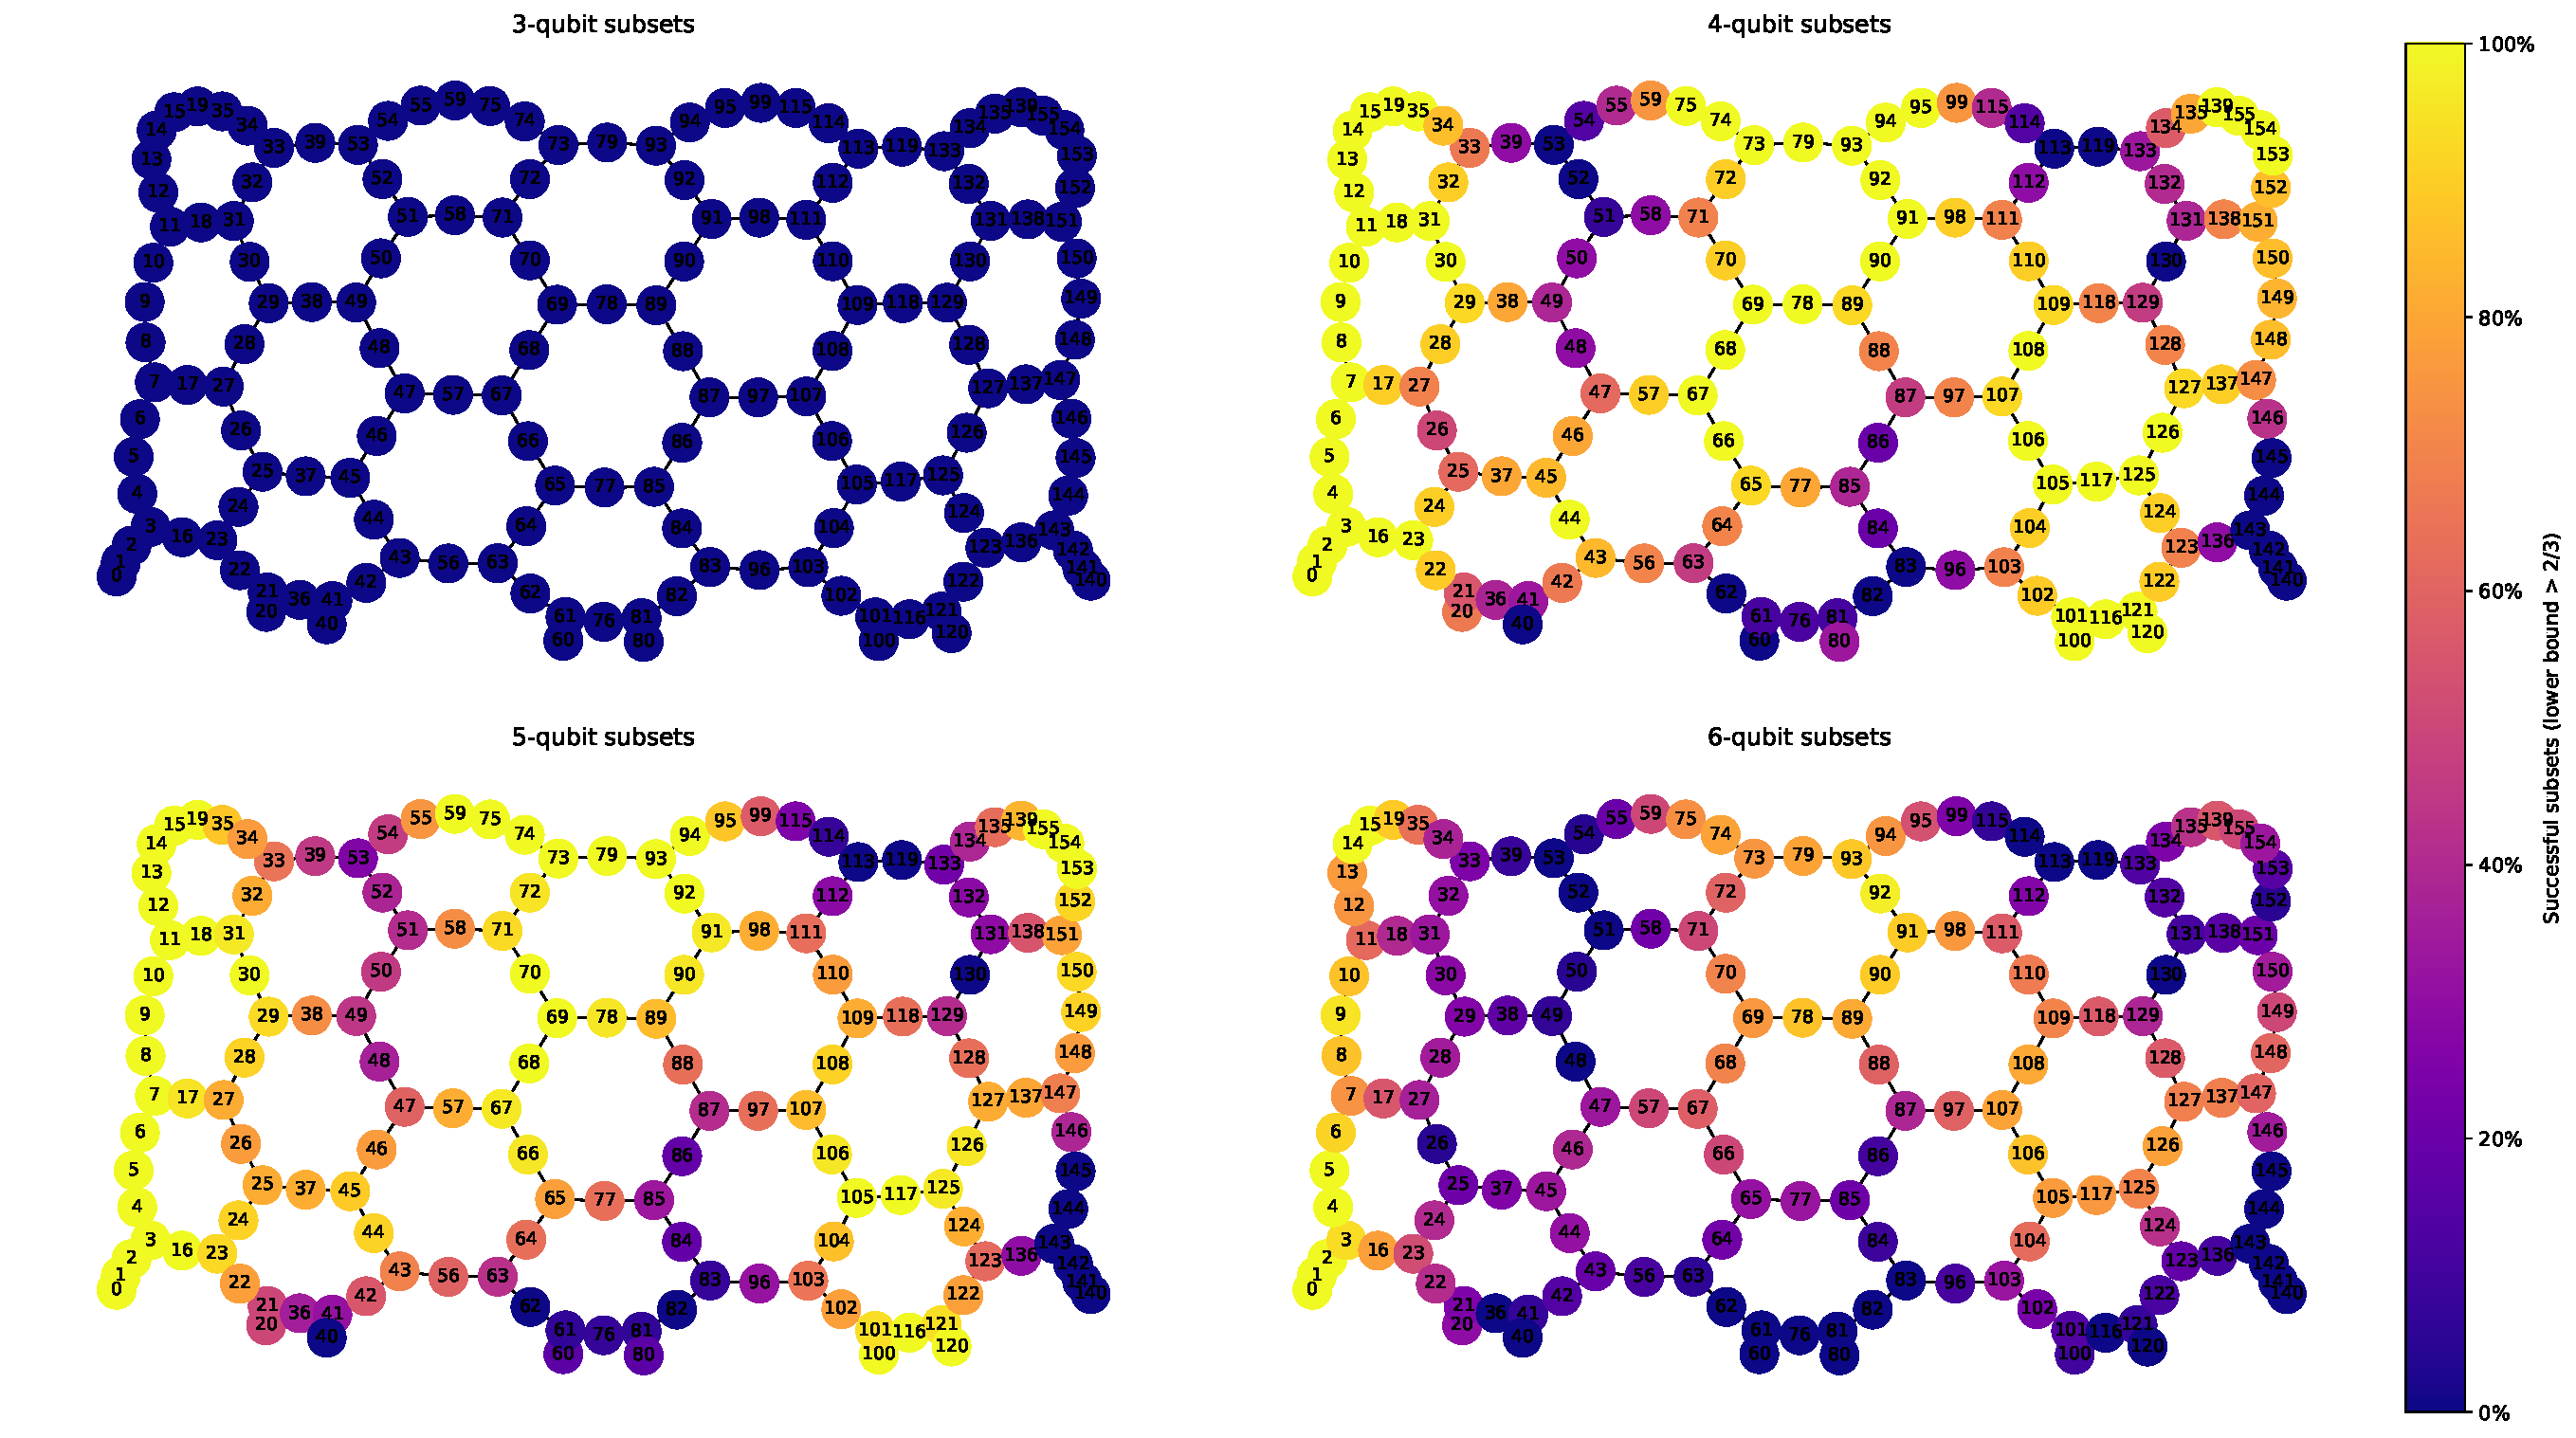
\includegraphics[width=\linewidth]{../results/success_fraction_grid.pdf}
		\small \textbf{Empiric probability that a qubit is part of a subset that passes the QV test over different subset sizes.} The success-fraction plot highlights that not all connected subsets of the same size perform equally well.

		\vspace{0.6em}

		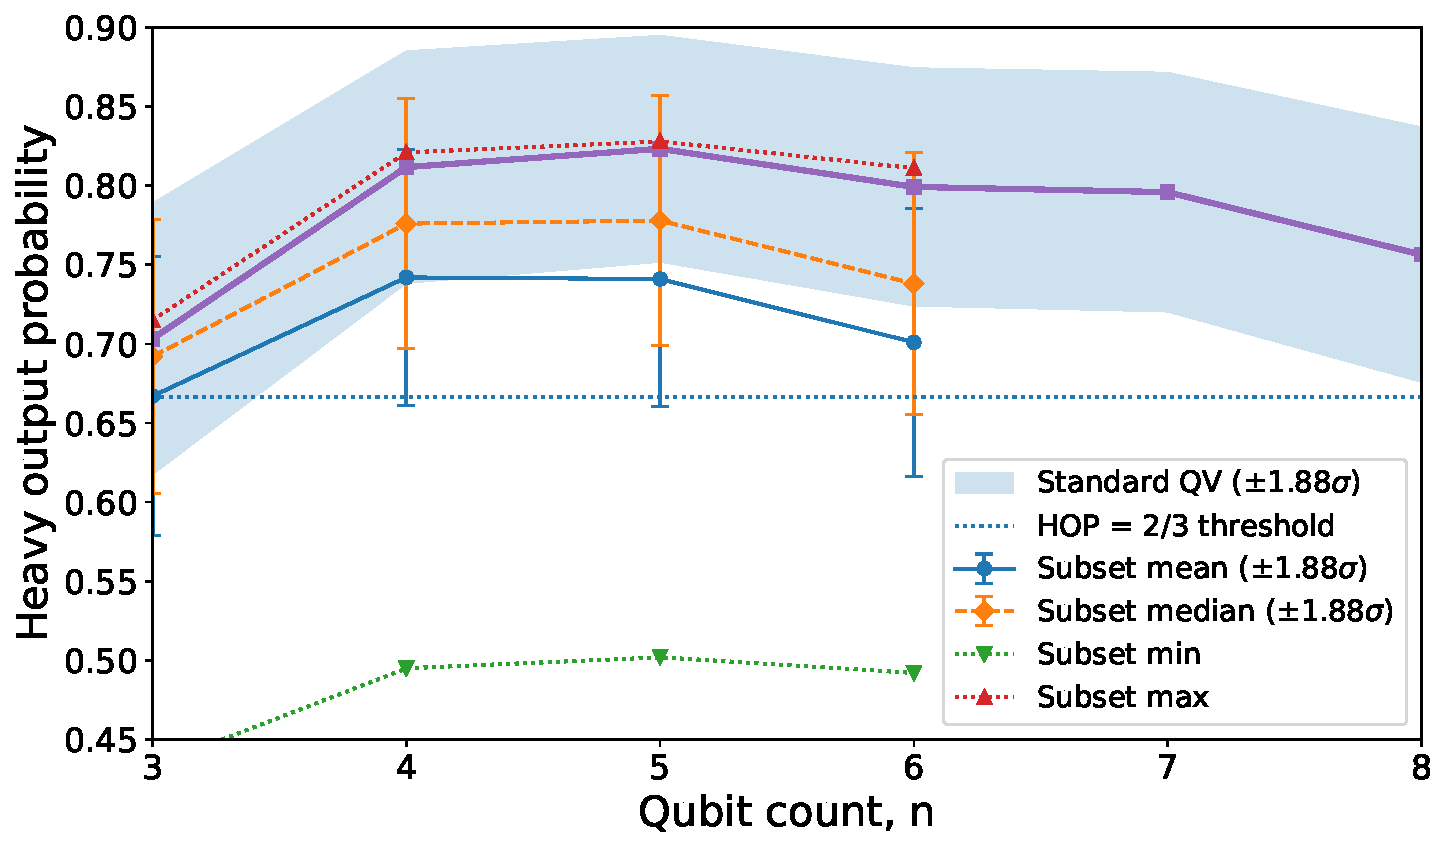
\includegraphics[width=\linewidth]{../results/qv_summary_stats.pdf}
		\small \textbf{Statistics of all subsets of different sizes, showing the mean and 97\% confidence interval of the heavy output probability.}

		\vspace{0.6em}

	\end{minipage}
	\hfill
	\begin{minipage}[t]{0.49\linewidth}
	\vspace{0pt}
		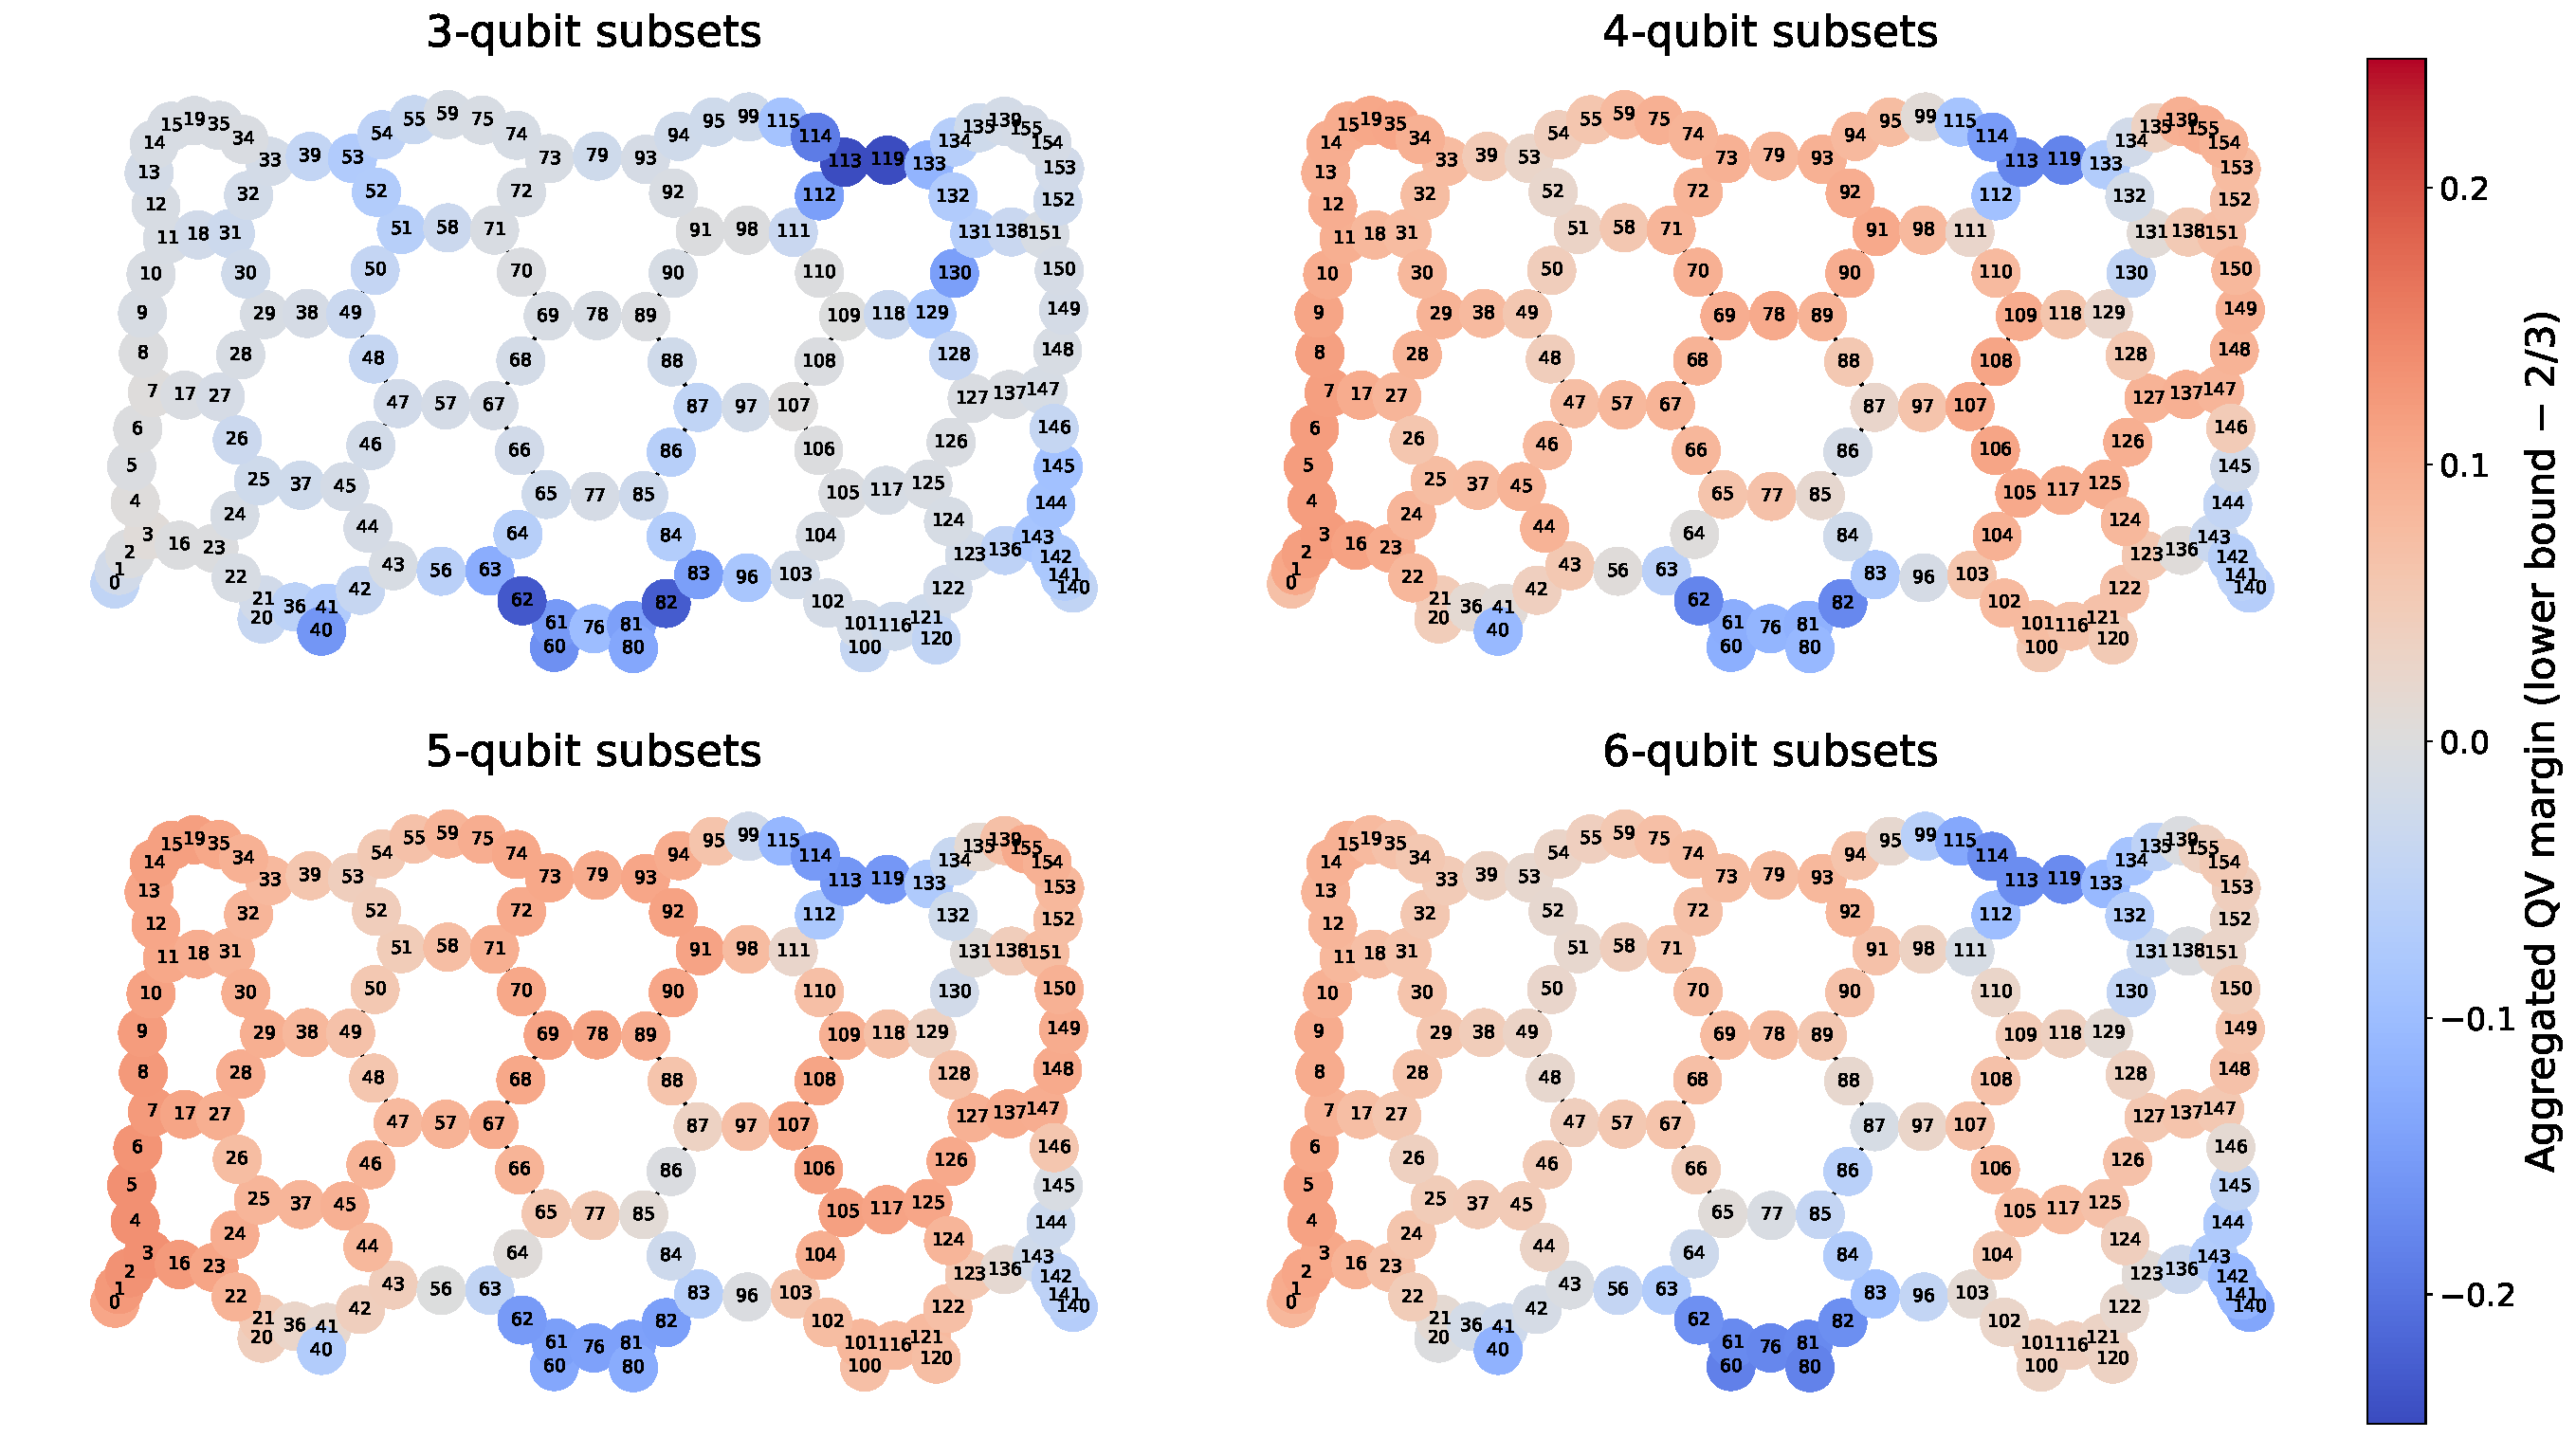
\includegraphics[width=\linewidth]{../results/aggregated_qv_grid.pdf}
		\small \textbf{Aggregated QV margin for each qubit, computed from all subsets containing it.} Each node participates in many connected subsets. For a given node $i$, we aggregate heavy output probabilities $\{\mu_j\}$ from all subsets $j$ containing $i$. \textbf{Mean score} is calculated as follows: $\bar{\mu}_i = \frac{1}{k_i} \sum_{j=1}^{k_i} \mu_j$. \textbf{Mean error} assumes independence $\sigma_i = \sqrt{\sum_{j=1}^{k_i} \sigma_j^2}\,/\,k_i$. \textbf{Lower confidence bound} takes into account the confidence interval of $2\sigma$. Finally, we compute the \textbf{QV margin} by subtracting the QV threshold of $\frac{2}{3}$ from the lower confidence bound. Note that subsets overlap, so errors are not fully independent; 
		the uncertainty is therefore slightly underestimated.

		\vspace{0.6em}
		
		\begin{tabular}{lllll}
\toprule
 & 3 & 4 & 5 & 6 \\
\midrule
\textbf{$T_1$ ($\mu$s)} & 0.11 & 0.10 & 0.08 & 0.09 \\
\textbf{$T_2$ ($\mu$s)} & 0.09 & 0.13 & 0.13 & 0.15 \\
\textbf{Meas0 prep1} & -0.58 & -0.47 & -0.41 & -0.36 \\
\textbf{Meas1 prep0} & -0.26 & -0.20 & -0.17 & -0.16 \\
\textbf{ID error} & -0.58 & -0.46 & -0.40 & -0.35 \\
\textbf{$X$ error} & -0.58 & -0.46 & -0.40 & -0.35 \\
\textbf{$\sqrt{X}$ error} & -0.58 & -0.46 & -0.40 & -0.35 \\
\textbf{Pauli-$X$ error} & -0.58 & -0.46 & -0.40 & -0.35 \\
\textbf{Measure error} & -0.44 & -0.34 & -0.29 & -0.25 \\
\bottomrule
\end{tabular}


		\vspace{0.6em}

		\small \textbf{Correlation of qubit-level metrics with the aggregated QV margin for each qubit.}

		\vspace{0.6em}

		
	\end{minipage}

	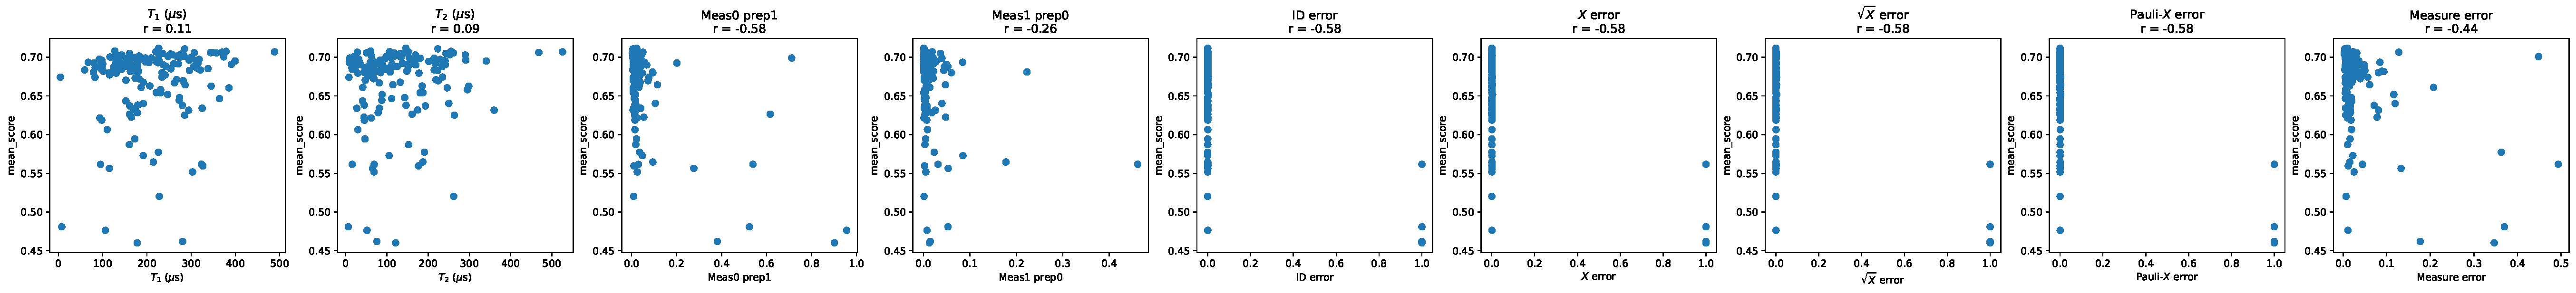
\includegraphics[width=\linewidth]{../results/node_metric_correlations_q3.pdf}

	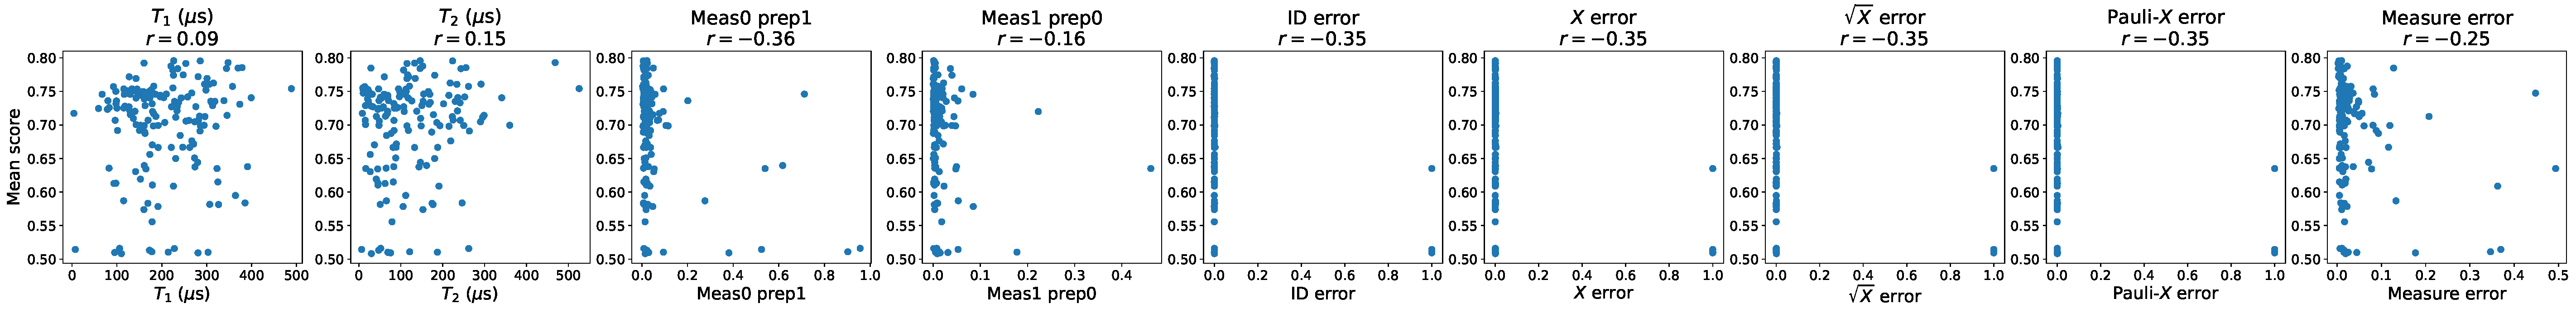
\includegraphics[width=\linewidth]{../results/node_metric_correlations_q6.pdf}

	\small \textbf{Correlation of qubit-level metrics with the aggregated QV margin for each qubit.} The first line conatins correlations for subsets of size 3, the second line for subsets of size 6. The correlation values are generally higher for smaller subsets, which is expected as they are more sensitive to noise and errors. The most strongly correlated metrics are readout error, measurement preparation errors, and gate errors, while coherence times ($T_1$ and $T_2$) show weaker correlations.

}


\end{poster}
\end{document}
